\documentclass{tufte-handout}
\usepackage{graphicx}
\usepackage{changepage}
\usepackage{amsmath}
\usepackage{float}

\definecolor{SolutionColor}{rgb}{0.5,0,0}
\newcommand{\solution}[1]{
\begin{adjustwidth}{1cm}{}
\textit{\color{SolutionColor} #1}
\end{adjustwidth}}
\usepackage{lipsum}
\newcommand\tab[1][1cm]{\hspace*{#1}}

\begin{document}

\begin{fullwidth} 
\section{MATH1010: Homework 1}
    \textit{Assigned January 10, 2022}
    \textbf{Due January 17, 2022}
    \vspace{.2cm}
    
\noindent\textit{Exercises taken from Easley and Kleinberg are reproduced here and referenced as \textbf{E\&K, Chapter X, Problem Y.}}    
    
\section*{\textbf{Exercise 1}}
\textit{E\&K, Chapter 3, Problem 1.}\\
In two to three sentences, explain what triadic closure is and how it plays a role in the formation of social networks. You can draw a picture if it's useful.
% \solution{
% You can type your answer here
% }
\section*{\textbf{Exercise 2}}
\textit{E\&K, Chapter 3, Problem 2.}\\
Consider the graph in the figure below, in which each edge-- except the edge connecting nodes $B$ and $C$-- is labeled as a strong tie (S) or a weak tie (W). \\
According to the theory of strong and weak ties, using the Strong Triadic Closure assumption, how would you expect the edge connecting $B$ and $C$ to be labeled? Give a brief explanation of your answer.
\begin{figure*}[!h]
    \centering
    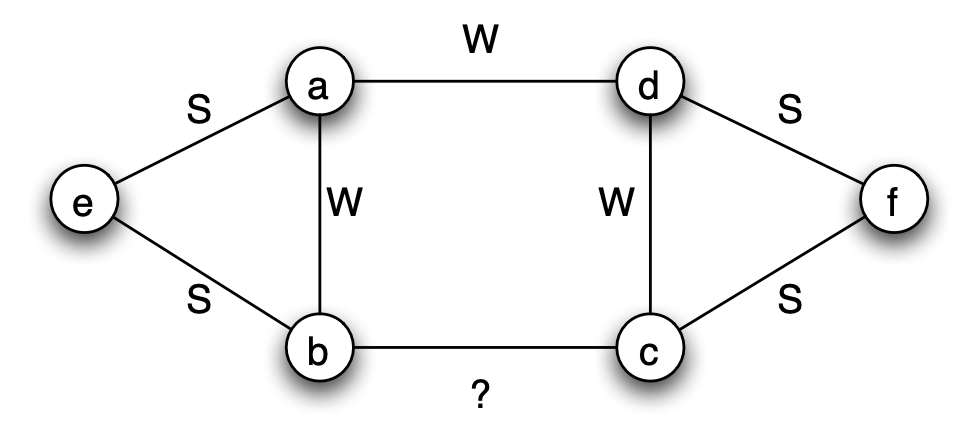
\includegraphics[width = .4\textwidth]{ek32.png}
    \caption{The graph for E\&K, Ch 3, Problem 2}
\end{figure*}
\section*{\textbf{Exercise 3}}
\textit{Betweenness in graphs}\\
In the following graph, find the edge with the highest \textit{betweenness}. What is its betweenness value? What would happen if the edge were removed?
\begin{figure*}[!h]
        \centering
        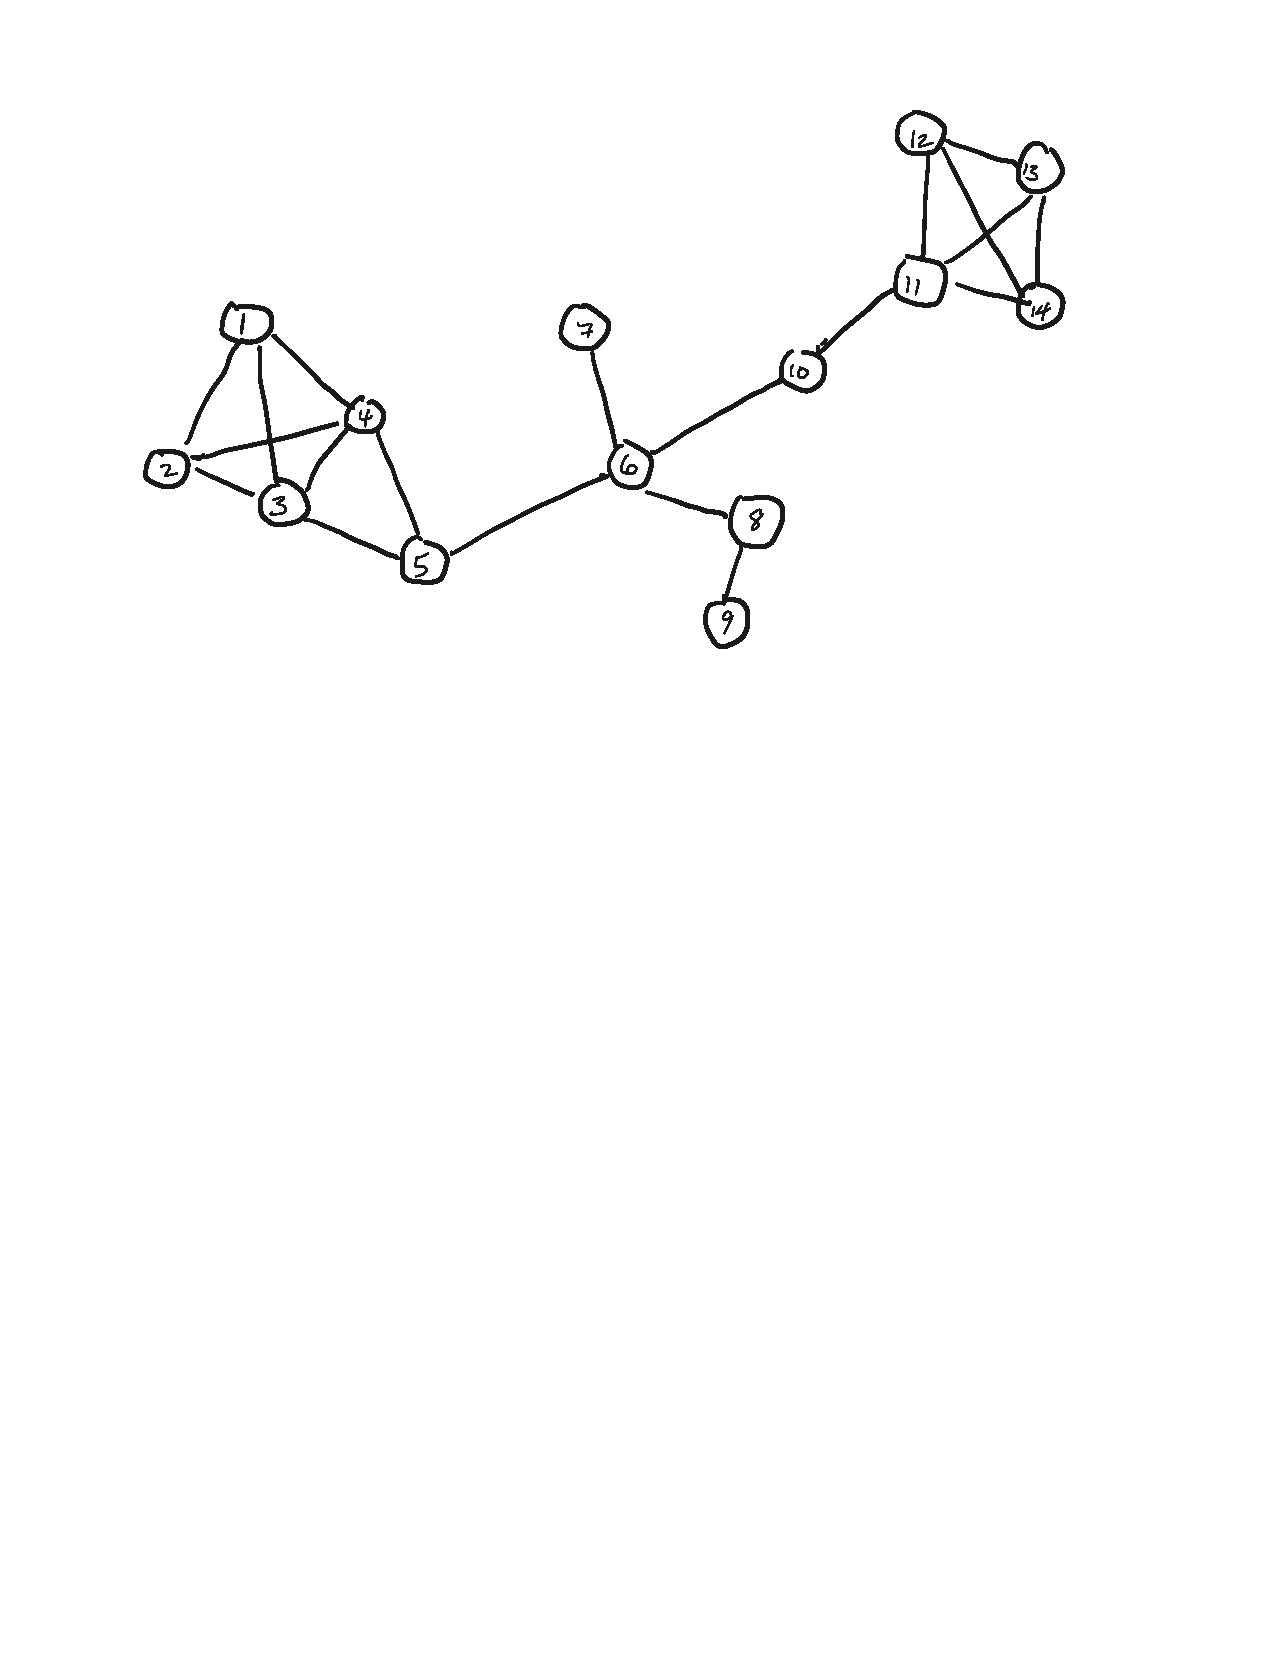
\includegraphics[width=.4\textwidth]{e3.pdf}
        \caption{The graph for exercise 3}
        \label{fig:e3}
    \end{figure*}
\newpage
\section*{\textbf{Exercise 4}}
\textit{Adjacency matrices}\\
\begin{enumerate}
    \item Write down the adjacency matrix for the following graph.
    \begin{figure*}[!h]
        \centering
        \includegraphics[width=.4\textwidth]{e41.pdf}
        \caption{The graph for exercise 4.1}
        \label{fig:e41}
    \end{figure*}
    \item Draw the graph for the following adjacency matrix. 
    $$
    \begin{bmatrix}
    0 & 0 & 0 & 1 & 0 & 1 \\
    0 & 0 & 1 & 1 & 0 & 0 \\
    0 & 1 & 0 & 0 & 1 & 1 \\
    1 & 1 & 0 & 0 & 0 & 0 \\
    0 & 0 & 1 & 0 & 0 & 1 \\
    1 & 0 & 1 & 0 & 1 & 0 
    \end{bmatrix}
    $$
\end{enumerate}
\section*{\textbf{Exercise 5}}
\textit{E\&K, Chapter 4, Problem 1.}\\
Consider the social network represented in Figure 4.20. Suppose that this social net- work was obtained by observing a group of people at a particular point in time and recording all their friendship relations. Now suppose that we come back at some point in the future and observe it again. According to the theories based on empirical studies of triadic closure in networks, which new edge is most likely to be present? (I.e. which pair of nodes, who do not currently have an edge connecting them, are most likely to be linked by an edge when we return to take the second observation?) Also, give a brief explanation for your answer.
\begin{figure*}[!h]
        \centering
        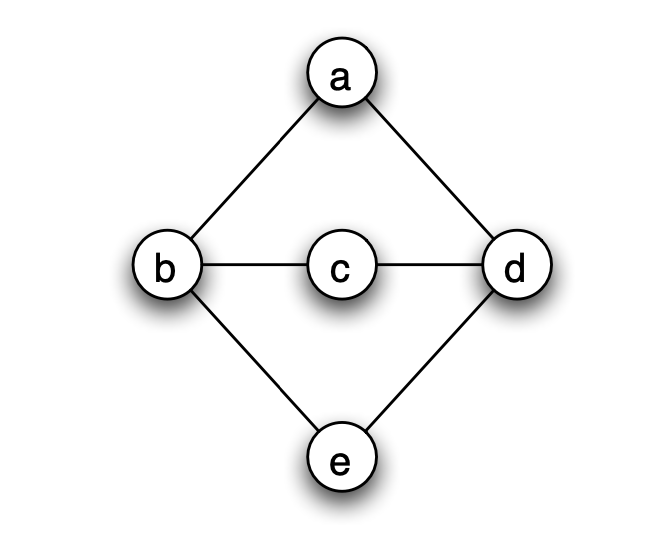
\includegraphics[width=.3\textwidth]{e420.png}
        \caption{The graph for E\&K, Chapter 4, Problem 1. Fig 4.20}
        \label{fig:e420}
    \end{figure*}
\end{fullwidth}
\end{document}
